% !TEX TS-program = pdflatexmk
\documentclass[12pt]{amsart}
\usepackage{multicol}
\usepackage{float}

%\usepackage[parfill]{parskip}    % Activate to begin paragraphs with an empty line rather than an indent

\usepackage[margin=1in]{geometry}


\usepackage{amsmath,amssymb,amsthm,latexsym,graphicx}
\usepackage[normalem]{ulem}
\usepackage{setspace} %used for doublespacing, etc.
\usepackage{hyperref}
\usepackage{cancel}
\usepackage[dvipsnames,usenames]{color}
\usepackage[all]{xy}
\usepackage{fancyhdr}
\pagestyle{fancy}
	\renewcommand{\headrulewidth}{0.5pt} % and the line
	\headsep=1cm
	
\DeclareGraphicsRule{.tif}{png}{.png}{`convert #1 `dirname #1`/`basename #1 .tif`.png}

%Some useful environments.
\newtheorem{theorem}{Theorem}
\newtheorem{corollary}[theorem]{Corollary}
\newtheorem{conjecture}[theorem]{Conjecture}
\newtheorem{lemma}[theorem]{Lemma}
\newtheorem{proposition}[theorem]{Proposition}
\newtheorem{definition}[theorem]{Definition}
\newtheorem{example}[theorem]{Example}
\newtheorem{axiom}{Axiom}
\theoremstyle{remark}
\newtheorem{remark}{Remark}
\newtheorem*{exercise}{Exercise}%[section]

%Some useful shortcuts for our favorite fields
\def\RR{\ensuremath{\mathbb R}} %Note, you can use these WITHOUT entering math mode
\def\NN{\ensuremath{\mathbb N}}
\def\ZZ{\ensuremath{\mathbb Z}}
\def\QQ{{\ensuremath\mathbb Q}}
\def\CC{\ensuremath{\mathbb C}}
\def\EE{{\ensuremath\mathbb E}}

%Some useful shortcuts for formatting lists
\newcommand{\bc}{\begin{center}}
\newcommand{\ec}{\end{center}}
\newcommand{\be}{\begin{enumerate}}
\newcommand{\ee}{\end{enumerate}}
\newcommand{\bi}{\begin{itemize}}
\newcommand{\ei}{\end{itemize}}

%Some useful shortcuts for formatting mathematical symbols
\newcommand{\ol}[1]{\overline{#1}}
\newcommand{\oimp}[1]{\overset{#1}{\iff}} %labeled iff symbol
\newcommand{\bv}[1]{\ensuremath{ \vec{\mathbf{#1}}} } %makes a vector.
\newcommand{\mc}[1]{\ensuremath{\mathcal{#1}}} %put something in caligraphic font
\newcommand{\mpg}[1]{\marginpar{ #1}} %to put comments in margins
\newcommand{\bsl}[1]{\texttt{\symbol{92}{\em #1}}} %for backslashes.
\newcommand{\normale}{\trianglelefteq}
\newcommand{\normal}{\triangleleft}

%Code for formatting the proofs a little nicer for submitted homework
\makeatletter
\renewenvironment{proof}[1][\proofname]{\par\doublespacing
  \pushQED{\qed}%
  \normalfont \topsep6\p@\@plus6\p@\relax
  \list{}{%
    \settowidth{\leftmargin}{\itshape\proofname:\hskip\labelsep}%
    \setlength{\labelwidth}{0pt}%
    \setlength{\itemindent}{-\leftmargin}%
  }%
  \item[\hskip\labelsep\itshape#1\@addpunct{:}]\ignorespaces
}{%
  \popQED\endlist\@endpefalse
  \singlespacing
}
\makeatother


%Commenting tools. You can ignore this stuff unless we're exchanging materials where I'm commenting in detail on how you are writing/using LaTeX.
\usepackage{soul}
\definecolor{highlight}{rgb}{1,0.6,0.6}
\sethlcolor{highlight}
\newcommand{\hlm}[1]{\colorbox{highlight}{$\displaystyle #1$}}
\newtheoremstyle{mycomment}{\topsep}{-0in}{\small \itshape \sffamily}{}{\small \itshape\sffamily}{:}{.5em}{}
\theoremstyle{mycomment}
\newtheorem*{acomment}{\color{BrickRed}{Comment}}
\newcommand{\com}[1]{{\color{OliveGreen}\begin{acomment}{#1} %#2 \color{black} 
\end{acomment}\noindent}}
%\newcommand{\com}[1]{{\color{BrickRed}{\\ Comment:}\color{OliveGreen}{#1} \\}}
\newcommand{\red}[1]{{\color{BrickRed} #1}}
\newcommand{\blue}[1]{{\color{MidnightBlue}#1}}
\newcommand{\green}[1]{{\color{OliveGreen}#1}}
\newcommand{\mwrong}[2]{\red{\cancel{#1}}\green{#2}}
\newcommand{\wrong}[2]{\red{\sout{#1}}\green{#2}}
\definecolor{OliveGreen}{rgb}{.3,.5,.2}
\definecolor{MidnightBlue}{rgb}{.3,.4,.6}
\newcommand{\pts}[1]{\hfill\blue{{#1}/5}}

\chead{MATH 631F}
\pagestyle{fancy}
%Modify these items:
\rhead{\emph{Stefano Fochesatto}}
\lhead{\emph{HW \#4 --- \today}}

\DeclareMathOperator{\lcm}{lcm}
\begin{document}

\thispagestyle{fancy}
\author{Coordinator: Coordinator's Name}


%3.1 1, 3, 4, 5, 7, 22, 24, 28, 31, 35, 36.
%3.1 37, 40, 41, 42.
%3.2 4, 5, 8, 10, 16, 22, 23. 





\section*{\textbf{Section 2.5} - My solutions from Group HW}


\begin{exercise}[\textbf{2.5.6c}] Use the given lattices to help find the centralizer of every element in $S_3$
  \begin{figure}[H] %\usepackage{float}
    \begin{center}
      \caption{Lattice Diagram for $S_{3}$}
      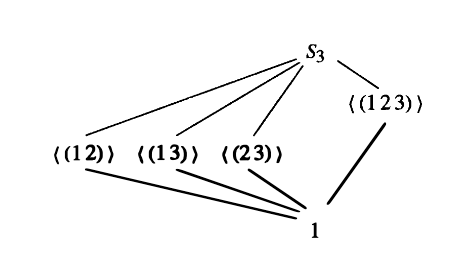
\includegraphics[width=.5\textwidth]{Sthree.png}
    \end{center}
  \end{figure} 
  \begin{proof}[Solution:] Clearly $C_{S_3}(1) = S_3$. Seeing how the centralizer of an element $x \in S_3$ is a subgroup 
    of $S_3$ containing $x$, by the way the lattice diagram is structured, $C_{S_3}((x))$ must be equal to either $\langle (x)\rangle$ or $S_3$.\\\\
    Consider $(12)$ and note that $(13)(12)(13) = (23)$, therefore $(13) \not\in C_{S_3}((12))$. Thus $C_{S_3}((12)) = \langle (12)\rangle$.\\\\
    Consider $(13)$ and note that $(12)(13)(12) = (23)$, therefore $(12) \not\in C_{S_3}((13))$. Thus $C_{S_3}((13)) = \langle (13)\rangle$.\\\\
    Consider $(23)$ and note that $(13)(23)(13) = (12)$, therefore $(13) \not\in C_{S_3}((23))$. Thus $C_{S_3}((23)) = \langle (23)\rangle$.\\\\
    Consider $(132)$ and note that $(13)(132)(13) = (123)$, therefore $(13) \not\in C_{S_3}((132))$. Since $(132) = (123)^2$, $C_{S_3}((132)) = C_{S_3}((123)) = \langle (123)\rangle$. 
  \end{proof}
\end{exercise}
\vspace{.15in}


\begin{exercise}[\textbf{2.5.8}]
  \noindent
  \begin{enumerate}
    \item Find the normalizer of each subgroup in $S_3$.
    \begin{figure}[H] %\usepackage{float}
      \begin{center}
        \caption{Lattice Diagram for $S_{3}$}
        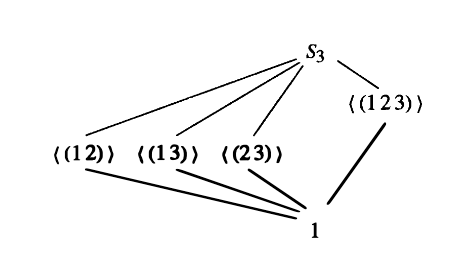
\includegraphics[width=.4\textwidth]{Sthree.png}
      \end{center}
    \end{figure} 
    \begin{proof}[Solution:]
      Clearly $N_{S_3}{\langle 1\rangle} = S_3$ and $N_{S_3}{\langle  S_3 \rangle} = S_3$. Similarly to the previous problem, since the normalizer of subgroup contains the subgroup,  and because of the structure of the lattice diagram for any subgroup $G$, 
      either $N_{S_3}(G) = G$ or $N_{S_3}(G) = S_3$.\\
    Consider $\langle 12\rangle$ and note that $(13)(12)(13) = (23)$. Since $(23) \not\in (\langle (12)\rangle)$ we know that $(13) \not\in N_{S_3}(\langle (12)\rangle)$ and therefore $N_{S_3}(\langle (12)\rangle) = \langle (12)\rangle$.\\\\
    Consider $\langle 13\rangle$ and note that $(12)(13)(12) = (23)$. Since $(23) \not\in (\langle (13)\rangle)$ we know that $(12) \not\in N_{S_3}(\langle (13)\rangle)$ and therefore $N_{S_3}(\langle (13)\rangle) = \langle (13)\rangle$.\\\\
    Consider $\langle 23\rangle$ and note that $(13)(23)(13) = (12)$. Since $(12) \not\in (\langle (23)\rangle)$ we know that $(13) \not\in N_{S_3}(\langle (23)\rangle)$ and therefore $N_{S_3}(\langle (23)\rangle) = \langle (23)\rangle$.\\\\
    Finally consider $\langle (123)\rangle = \{1, (123), (132)\}$, and note that
    \begin{equation*}
      (12)(123)(12) = (132),
    \end{equation*}
    \begin{equation*}
      (12)(132)(12) = (123).
    \end{equation*}
    Therefore, $(12) \in N_{S_3}(\langle (123)\rangle)$, and since $(12) \not\in \langle (123)\rangle$ we know that $N_{S_3}(\langle (123)\rangle) = S_3$. 
    \end{proof}
    \vspace{.15in}

    \item Find the normalizer of each subgroup in $Q_8$\\
   \begin{figure}[H] %\usepackage{float}
      \begin{center}
        \caption{Lattice Diagram for $Q_{8}$}
        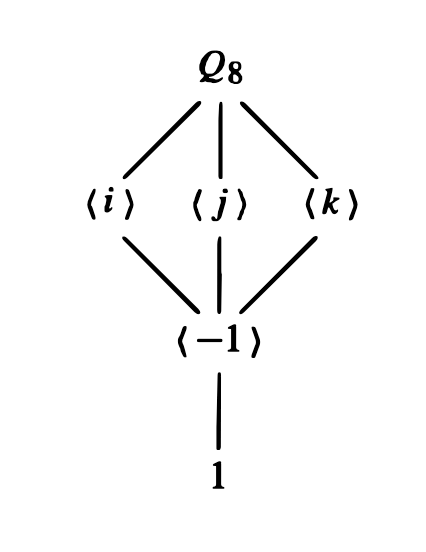
\includegraphics[width=.3\textwidth]{Qeight.png}
      \end{center}
    \end{figure} 
    \begin{proof}[Solution:] Clearly $N_{Q_8}(\langle 1\rangle) = Q_8$ and $N_{Q_8}(\langle  Q_8 \rangle) = Q_8$. Let $a\in Q_8$ and note that,
      $a(-1)a^{-1} = a(-1)(-1)a = a^2 = -1 \in \langle -1\rangle $. Thus  $N_{Q_8}(\langle -1\rangle) = Q_8$. Since the normalizer of subgroup contains the subgroup, and because of the structure of the lattice diagram for subgroups $G = \{\langle  i \rangle, \langle  j \rangle, \langle  k \rangle\}$, 
      either $N_{Q_8}(G) = G$ or $N_{Q_8}(G) = Q_8$.\\
      Consider $\langle  i \rangle$ and note that $ji(-j) = (-k)(-j) = -i \in \langle i\rangle $  and $j-i(-j) = (j)(k) = i \in \langle i\rangle $. Therefore $j \in N_{Q_8}(\langle  i \rangle)$, thus $N_{Q_8}(\langle  i \rangle) = Q_8$. \\\\
      Consider $\langle  j \rangle$ and note that $ij(-i) = (k)(-i) = -j \in \langle j\rangle $  and $i-j(-i) = (i)(-k) = j \in \langle j\rangle $. Therefore $j \in N_{Q_8}(\langle  j \rangle)$, thus $N_{Q_8}(\langle  j \rangle) = Q_8$. \\\\
      Consider $\langle  k \rangle$ and note that $ik(-i) = (-j)(-i) = -k \in \langle k\rangle $  and $i-k(-i) = (i)(j) = k \in \langle k\rangle $. Therefore $j \in N_{Q_8}(\langle  k \rangle)$, thus $N_{Q_8}(\langle  k \rangle) = Q_8$. 
    \end{proof}
  \end{enumerate}
\end{exercise}
\vspace{.15in}


\section*{\textbf{Section 3.1}}


\begin{exercise}[\textbf{3.1.1}] Let $\varphi : G \to H$ be a homomorphism and let $E$ be a subgroup of $H$. Prove that $\varphi^{-1}(E) \leq G$. 
  If $E\lhd H$ prove that $\varphi^{-1}(E)\lhd G$. Deduce that $ker \varphi \lhd G$.
  \begin{proof} Suppose $\varphi : G \to H$ is a homomorphism and consider $E$, a subgroup of $H$. By properties of homomorphisms $1 \in \varphi^{-1}(E)$. Now consider 
    $x, y \in \varphi^{-1}(E)$. By definition there exists some $a, b \in E$ such that $\varphi(x) = a$, and $\varphi(y) = b$. Consider $xy$ and note that since $\varphi$ is a homomorphism, 
    $\varphi(xy) = \varphi(x)\varphi(y) = ab$. Since $E$ is a group $ab \in E$ and therefore by definition $xy \in \varphi^{-1}(E)$. By properties of homorphisms we know that 
    $\varphi(x^{-1}) = \varphi(x)^{-1} = a^{-1}$, since $a^{-1} \in E$ we know that $x^{-1} \in \varphi^{-1}(E)$. Thus $\varphi^{-1}(E) \leq G$. \\

    Suppose $E\lhd H$. By definition $heh^{-1} \in E$, for all $h \in H$ and $e \in E$. Let $g \in G$ and $a \in \varphi{-1}(E)$. Note 
    $\varphi(gag^{-1}) = \varphi(g)\varphi(a)\varphi(g)^{-1} = heh^{-1}$. Since $E\lhd H$, $heh^{-1} \in E$ and therefore $\varphi^{-1}(E)\lhd G$.\\

   Let $E$ be the trivial subgroup which is also normal in $H$. It follows that $\varphi^{-1}(E) = \ker \varphi$, and by the previous result $ker \varphi \lhd G$. 
  \end{proof}

\end{exercise}
\vspace{.15in}


%%%% Example Needed maybe Q_8
\begin{exercise}[\textbf{3.1.3}] Let $A$ be an abelian group and let $B$ be a subgroup of $A$. Prove that $A/B$ is abelian. Give an 
  example of a non-abelian group $G$ containing a proper normal subgroup $N$ such that $G/N$ is abelian.\\

    \begin{proof} Suppose $A$ be an abelian group and let $B$ be a subgroup of $A$. Consider $x, y \in A$, and note that 
      $xB, yB \in A/B$. Since $B$ is a subgroup of $A$ we know that $xByB = (xy)B$, and since $A$ is abelian, 
      \begin{equation*}
        xByB = (xy)B = (yx)B = yBxB.
      \end{equation*}
      Therefore $A/B$ is abelian.
      \end{proof}
      Maybe for an example consider $Q_8$ with normal subgroup $\langle -1 \rangle$. 

\end{exercise}
\vspace{.15in}


\begin{exercise}[\textbf{3.1.4}] Prove that in the quotient group $G/N$, $(gN)^\alpha = g^{\alpha}N$ for all 
  $\alpha \in \ZZ$.
    \begin{proof} Suppose $N$ is a subgroup of $G$ and consider the quotient group $G/N$. By Proposition 5 we know that, 
      $g_1N \cdot g_2N = (g_1g_2)N$ is a well defined operation. What follows is that $(gN)^{-1} = g^{-1}N$. Therefore for $\alpha \in \ZZ$, 
      \begin{equation*}
        (gN)^\alpha = g_1N \cdot g_2N \cdot ... \cdot g_\alpha N = (g_1g_2...g_\alpha)N = g^{\alpha}N.
      \end{equation*}
    \end{proof}

\end{exercise}
\vspace{.15in}

\begin{exercise}[\textbf{3.1.5}] Use the preceding exercise to prove that the order of the element $gN$ in $G/N$ is $n$, where $n$ is the smallest positive integer such that $g^n \in N$. 
    \begin{proof} Suppose $gN \in G/N$, and let $n$ be the smallest positive integer such that $g^n \in N$. By the previous 
      problem we know that $(gN)^n = g^nN = N$ since $g^n \in N$. Thus $|gN| \leq n$. Suppose that $(gN)^i = N$, by definition it follows 
      that $(gN)^i = g^iN = N$, therefore $g^i \in N$. Note that $n$ is the smallest such integer such that and therefore $|gN| \geq n$. 
      Thus $|gN| = n$.
    \end{proof}

\end{exercise}
\vspace{.15in}


\begin{exercise}[\textbf{3.1.7}]Define $\pi: \RR^2 \to \RR$ by $\pi((x, y)) = x+y$. Prove that $\pi$ is a surjective homomorphism 
  and describe the kernel and fibers of $\pi$ geometrically
    \begin{proof} Suppose $\pi: \RR^2 \to \RR$ by $\pi((x, y)) = x+y$. Let $(x, y), (a,b) \in \RR^2$ and consider $\pi((x, y) + (a, b)) = \pi((a + x, b + y)) = a + x + b + y = a + b + x + y = \pi((a, b))\pi((x, y))$. 
      Thus $\pi$ is a homomorphism. Let $x \in \RR$, consider $(x, 0) \in \RR^2$ and note $\pi((x, 0)) = x + 0 = x$ and thus $\pi$ is a surjection.\\
      Now consider the kernel of $\pi$, and note that $\ker(\pi) = \{(x, -x) \in \RR^2| x \in \RR\}$ since $\pi(x, -x) = x - x = 0$ which is the identity in $\RR$. 
      Geometrically this is the line $y = -x$. Recall that the fibers of $\pi$ for a given element $a \in \RR$ is the set of all 
      $\phi^{-1}(a) = \{(x, y) \in \RR^2: x + y = a\}$. Thus fibers of $\pi$ are of the form $y = a - x$, and geometrically represent lines parallel to the kernel. 
    \end{proof}
\end{exercise}
\vspace{.15in}


\begin{exercise}[\textbf{3.1.22}]
  \begin{enumerate}
    \item[a.] Prove that if $H$ and $K$ are normal subgroups of group $G$ then their intersection $H \cap K$ is
    also a normal subgroup of $G$.
    \begin{proof} Suppose $H$ and $K$ are normal subgroups of group $G$. Suppose $a, b \in H\cap K$ clearly $ab^{-1} \in H\cap K$ since 
      $H$ and $K$ are subgroups and both contain $a, b$. Hence $H \cap K$ is a subgroup. Let $g \in G$ and $a \in H \cap K$ clearly 
      $gag^{-1} \in H$ since $H$ is normal in $G$, and $gag^{-1} \in K$ since $K$ is normal in $G$. Thus $gag^{-1} \in H\cap K$ and therefore 
      $H \cap K$ is a normal subgroup of $G$. 
    \end{proof}
    
    \vspace{.15in}
    \item[b.] Prove that the intersection of an arbitrary nonempty collection of normal subgroups of a group is 
    a normal subgroup.
    \begin{proof} Suppose $\mathcal{H}$ is a family of nonempty normal subgroups in a group $G$. Consider the following 
    $a \in \cap \mathcal{H}$. Clearly for $g \in G$, $gag^{-1} \in H_i$ for all $H_i \in \mathcal{H}$ since $\mathcal{H}$ 
    is a family of normal subgroups. Thus by definition it follows that,  $gag^{-1} \in \cap \mathcal{H}$. 
    \end{proof}
  \end{enumerate}
\end{exercise}
\vspace{.15in}


\begin{exercise}[\textbf{3.1.24}] Prove that if $N$ is a normal subgroup of $G$ and $H$ is any subgroup of $G$ then $N\cap H$
  is a normal subgroup of $H$.
  \begin{proof} Suppose $N$ is a normal subgroup of $G$ and $H$ is any subgroup of $G$. Let $a, b \in N\cap H$, clearly 
    $ab^{-1} \in  N\cap H$, hence $N\cap H \leq H$. Note that since $N$ is normal in $G$ and $H$ is a subgroup for all $h \in H$
    $hah^{-1} \in N$. Since $a \in H$ and $H$ is a subgroup we know that $hah^{-1} \in H$. Thus $hah^{-1} \in N\cap H$ and therefore 
    $N\cap H$ is normal in $H$. 
  \end{proof}
\end{exercise}
\vspace{.15in}


\begin{exercise}[\textbf{3.1.28}] Let $N$ be a finite subgroup of a group $G$ and assume $N = \langle S\rangle $ for some subset $S$ of $G$. 
  Prove that an element $g \in G$ normalizes $N$ if and only if $gSg^{-1} \subseteq N$.
  \begin{proof} Let $N$ be a finite subgroup of a group $G$ and $N = \langle S\rangle $ for some subset $S$ of $G$. Suppose $g \in G$ normalizes $N$. By definition
    it follows that for $g \in G$, $gng^{-1} \in N$. By definition $N$ is also the intersection of all subgroups containing $S$, hence $S \subseteq N$
    and since $S$ is a subset of $G$ for all $s \in S$, $gsg^{-1} \in N$. Thus $gSg^{-1} \subseteq N$. \\

    Now suppose $gSg^{-1} \subseteq N$. Since $N$ is the group generated by $S$ by definition every $n$ is equal to some unique, finite product of the 
    elements of $S$, hence $n = s_1^{\alpha_1}s_2^{\alpha_2}\dots s_k^{\alpha_k}$. Consider $gng^{-1}$ and note that by substitution, 
    \begin{align*}
      gng^{-1} &= gs_1^{\alpha_1}s_2^{\alpha_2}\dots s_k^{\alpha_k}g \\
      &= gs_1^{\alpha_1}(g^{-1}g)s_2^{\alpha_2}\dots (g^{-1}g)s_k^{\alpha_k}g^{-1}\\ 
      &= (gs_1^{\alpha_1}g^{-1})(gs_2^{\alpha_2}g^{-1})\dots (gs_k^{\alpha_k}g^{-1})\\ 
      &= (gs_1g^{-1})^{\alpha_1}(gs_2g^{-1})^{\alpha_2}\dots (gs_kg^{-1})^{\alpha_k}.
    \end{align*}
    Since $gSg^{-1} \subseteq N$ and $N$ is a group, $gng^{-1} = (gs_1g^{-1})^{\alpha_1}(gs_2g^{-1})^{\alpha_2}\dots (gs_kg^{-1})^{\alpha_k} \in N$. Thus $g \in G$ normalizes $N$.
    \end{proof}
\end{exercise}
\vspace{.15in}


\begin{exercise}[\textbf{3.1.31}] Prove that if $H \leq G$ and $N$ is a normal subgroup of $H$ then $H \leq N_G(N)$. Deduce that $N_G(N)$ is the largest subgroup of $G$ in which $N$ is normal (i.e., is the join of all 
  subgroups $H$ for which $N \trianglelefteq H$)
  \begin{proof} Suppose $H \leq G$ and $N$ is a normal subgroup of $H$. Consider $h \in H$, since $N$ is 
    a normal subgroup of $H$ we know that $hNh^{-1} = N$ so clearly $h \in N_G(N)$. Therefore $H$ is a subgroup contained in $N_G(N)$ and thus $H \leq N_G(N)$.\\
    
    Consider the set $B$ of all subgroups $H$ of $G$ such that $N \trianglelefteq H$. Note that by definition $N_G(N) \in B$. By the previous result every $H \in B$ has the property that $H \leq N_G(N)$ therefore $N_G(N)$ must be the largest subgroup of $G$ normal to $N$. 
  \end{proof}
\end{exercise}
\vspace{.15in}


\begin{exercise}[\textbf{3.1.35}]  Prove that $SL_n(F) \trianglelefteq GL_N(F)$ and describe the isomorphism 
  type of the quotient group
  \begin{proof} Clearly the group $SL_n(F)$, the set of all $NxN$ matrices with determinant 1 over the field $F$, it is contained within the 
    set of all $NxN$ matrices with nonzero determinant over the field $F$, hence $SL_n(F) \leq GL_N(F)$. Consider $X \in SL_n(F)$ and $Y \in GL_n(F)$ and note that by properties of determinant, 
    \begin{equation*}
      \det(YXY^{-1}) = \det(Y)\det(X)\det(Y^{-1}) = \det(Y)(1)\dfrac{1}{\det(Y)} = 1.
    \end{equation*}
    Therefore by definition $YXY^{-1} \in SL_n(F)$. Thus $SL_n(F) \trianglelefteq GL_N(F)$.\\
    Consider the map $f: GL_n(F) \to (F^*)^x$ defined by $f(X) = det(X)$. Let $A, B \in GL_n(F)$ and note that $f(AB) = det(AB) = det(A)det(B) = f(A)f(B)$. By the first homomorphism theorem we know that $ker(f) \trianglelefteq GL_n(F)$ and $G_n(F)/ker(f) \cong f(GL_n(F))$. Note that since $A \in S_n(F)$ is defined as the set of matrices with $det(A) = 1$. Thus $G/ker(f) = G_n(F)/S_n(F)$. Also note that $f(GL_n(F)) = F^*$ by the definition of $GL_n(F)$, thus $G_n(F)/S_n(F) \cong F^*$. 
  \end{proof}

\end{exercise}
\vspace{.15in}


\begin{exercise}[\textbf{3.1.36} - Stefano Fochesatto] Prove that if $G/Z(G)$ is cyclic then $G$ is abelian. [If $G/Z(G)$ is cyclic 
  with generator $xZ(G)$, show that every element of $G$ can be written in the form $x^az$ for some integer $a \in \ZZ$ and some element $z \in Z(G)$.]
  \begin{proof} Suppose $G/Z(G) = \langle  xZ(G)\rangle$ for some fixed $x \in G$. Since $G/Z(G)$ is cyclic there exists some $a \in \ZZ$ such that for all $g \in G$, 
    \begin{equation*}
      gZ(G) = (xZ(G))^a = x^aZ(G). 
    \end{equation*}
    Now consider $a, b \in G$, and note since $Z(G)$ is a subgroup of $G$ we know $G/Z(G)$ forms a partition of $G$ and thus 
    $a$ and $b$ belong to some left coset of $Z(G)$. Therefore by the previous result there exists some 
    $\alpha, \beta \in \ZZ$ and $z_1, z_2 \in Z(G)$ such that $a = x^{\alpha}z_1$ and $b = x^{\beta}z_2$. Since $z_1, z_2$ are commute with every element in $G$, 
    \begin{equation*}
      ab = x^{\alpha}(z_1x^{\beta})z_2 = x^{\alpha + \beta}(z_1z_2) = x^{\alpha + \beta}z_2z_1 = x^{\beta}(x^{\alpha}z_2)z_1 = x^{\beta}z_2x^{\alpha}z_1 = ba
    \end{equation*}
  \end{proof}
\end{exercise}
\vspace{.15in}


\begin{exercise}[\textbf{3.1.37}] Let $A$ and $B$ be groups. Show that $\{(a, 1) | a \in A\}$ is a normal subgroup of $AxB$ and the 
  quotient of $A x B$ by this subgroup is isomorphic to $B$. 
  \begin{proof} Suppose $A$ and $B$ are groups. Let $X = \{(a, 1) | a \in A\}$, and consider $(a, b) \in AxB$, and $(x, 1)\in X$. Note that 
    $(a, b)(a, 1)(a, b)^{-1} = (a, b)(a, 1)(a^{-1}, b^{-1}) = (axa^{-1}, b1b^{-1}) = (axa^{-1}, 1)$. Since $A$ is a subgroup and $x \in A$,  
    $axa^{-1} \in A$ and therefore $(axa^{-1}, 1) \in X$. Thus $X \trianglelefteq A$. \\

    Consider $AxB/X$, and define the mapping $\varphi:AxB/X \to B$ by $\varphi((a, b)X) = b$.\\
    Let $(a, b)X = (\alpha, \beta)X$. Therefore it follows that the product $(a, b)(\alpha, \beta)^{-1} = (a, b)(\alpha^{-1}, \beta^{-1}) = (a\alpha^{-1}, b\beta^{-1}) \in X$. Thus $b\beta^{-1} = 1$ and $b = \beta$ so $\varphi$ is well defined.\\
    Note that $\varphi((a, b)X(\alpha, \beta)X) = \varphi((a, b)(\alpha, \beta)X) = \varphi((a\alpha, b\beta)X) = b\beta = \varphi((a, b)X)\varphi((\alpha, \beta)X)$. Thus $\varphi$ is a homomorphism.\\

    Let $\varphi((a, b)X) = \varphi((\alpha, b)X)$. Note that $(a, b)(\alpha b)^{-1} = (a\alpha, bb^{-1}) = (a\alpha, 1)$. By definition $(a\alpha, 1) \in X$ so $(a, b)X = (\alpha, b)X$. Thus $\varphi$ is injective. Clearly $\varphi$ is a surjection, let $b \in B$ since the domain is $AxB/X$ we can always construct an $(a, b)X$ such that $\varphi((a, b)X) = b$. 
  \end{proof}

\end{exercise}
\vspace{.15in}


\begin{exercise}[\textbf{3.1.40}] Let $G$ be a group, let $N$ be a normal subgroup of $G$ and let $\overline{G} = G/N$. Prove that 
  $\overline{x}$ and $\overline{y}$ commute in $\overline{G}$ if and only if $x^{-1}y^{-1}xy \in N$. 
  \begin{proof} Let $G$ be a group, $N \trianglelefteq G$, and $\overline{G} = G/N$.  Suppose for $\overline{x}, \overline{y} \in \overline{G}$, $\overline{x}\overline{y} = \overline{x}\overline{y}$. It follows that $xyN = yxN$ and for some $n_1, n_2 \in N$ we know that, 
    \begin{align*}
      xyn_1 &= yxn_2,\\
      (yx)^{-1}xyn_1 &= n_2,\\
      x^{-1}y^{-1}xy &= n_2n_1^{-1}.
    \end{align*}
    Since $N$ is a subgroup we know that $x^{-1}y^{-1}xy \in N$.\\
    Now suppose that  $x^{-1}y^{-1}xy \in N$. Let $n \in N$ and consider the following, 
    \begin{align*}
      x^{-1}y^{-1}xy &= n\\
      xy &= yxn\\
    \end{align*}
    Therefore $xy \in yxN$. Since $N$ is normal the cosets of $G/N$ partition $G$, and since  $xy \in yxN$ it must be the case that $xyN = yxN$. 
  \end{proof}

\end{exercise}
\vspace{.15in}


\begin{exercise}[\textbf{3.1.41}] Let $G$ be a group. Prove that $N = \langle x^{-1}y^{-1}xy | x, y, \in G \rangle$ is a normal subgroup of $G$.
  and $G/N$ is abelian.\\
  \begin{proof} Let $G$ be a group, and suppose that $N = \langle x^{-1}y^{-1}xy | x, y, \in G \rangle$. Consider $g \in G$. Note that for the generator of $N$, 
    $gx^{-1}y^{-1}xyg^{-1} =  gx^{-1}(g^{-1}g)y^{-1}(g^{-1}g)x(g^{-1}g)yg^{-1} = (gx^{-1}g^{-1})(gy^{-1}g^{-1})(gxg^{-1})(gyg^{-1}) = (gxg^{-1})^{-1}(gyg^{-1})^{-1}(gxg^{-1})(gyg^{-1})$
    Since $G$ is a group $gxg^{-1}, gyg^{-1} \in G$ therefore by definition $gx^{-1}y^{-1}xyg^{-1} \in N$. Thus $N \trianglelefteq G$.\\ 
    Since $x^{-1}y^{-1}xy \in N$ for all $x, y \in G$, and $N \trianglelefteq G$ by the previous exercise $G/N$ must be abelian. 
  \end{proof}

\end{exercise}
\vspace{.15in}



\begin{exercise}[\textbf{3.1.42}] Assume both $H$ and $K$ are normal subgroups of $G$ with $H \cap K = 1$. Prove that $xy = yx$.
  \begin{proof} Suppose both $H$ and $K$ are normal subgroups of $G$ and $H \cap K = 1$. Let $x \in H$ and $y \in K$. Consider the element $x^{-1}y^{-1}xy$. Note that since $x \in H$,  $y \in G$, and $H \trianglelefteq G$ we know that there exists some $x_1 \in H$ such that $x = yx_1y^{-1}$. By substitution we get, $x^{-1}y^{-1}(yx_1y^{-1})y = x^{-1}x_1 \in H$. Now note that since $y^{-1} \in K$, $x \in G$, and $K \trianglelefteq G$ there exists some $y_1 \in K$ such that $y^{-1} = xy_1x^{-1}$. By substitution we get that $x^{-1}y^{-1}xy = x^{-1}(xy_1x^{-1})xy = y_1y \in K$. Therefore it follows that $x^{-1}y^{-1}xy \in H \cap K$. Thus $x^{-1}y^{-1}xy = 1$ and clearly $xy = yx$. 
  \end{proof}
\end{exercise}
\vspace{.15in}


\section*{\textbf{Section 3.2}}


\begin{exercise}[\textbf{3.2.4}]Show that if $|G| = pq$ for some primes $p$ and $q$ then either $G$ is abelian or $Z(G) = 1$\\
  \begin{proof} Consider $G$ such that $|G| = pq$ for some primes $p$ and $q$. Since $|G| = pq$ By Lagrange's Theorem it follows that $|Z(G)| = 1, p, q, pq$. Clearly if $|Z(G)| = 1$ then $Z(G) = 1$ and we are done, similarly if $|Z(G)| = pq$ then $Z(G) = G$ and therefore $G$ is abelian. Without
    loss of generality let $|Z(G)| = p$. By Lagrange's Theorem $|G/Z(G)| = |G|/|Z(G)| = pq/p = q$. Since $|G/Z(G)|$ is of prime order then $G/Z(G)$ must be cyclic. By 3.1.36 if $G/Z(G)$ is cyclic then $G$ is abelian. 
    \end{proof}
\end{exercise}
\vspace{.15in}



\begin{exercise}[\textbf{3.2.5}] Let $H$ be a subgroup of $G$ and fix some element $g \in G$.
  \begin{enumerate}
    \item[a] Prove that $gHg^{-1}$ is a subgroup of $G$ of the same order as $H$.\\
    \begin{proof} Suppose $H$ is a subgroup of $G$ and fix some element $g \in G$. Consider the group $gHg^{-1}$. Clearly this 
      group is non empty, as it contains the identity. Let $a, b \in gHg^{-1}$ for some $h_a, h_b \in H$ such that $a = gh_ag^{-1}$ and 
      $b = gh_bg^{-1}$. Note that $ab^{-1} = gh_ag^{-1}gh_b^{-1}g^{-1} = gh_ah_b^{-1}g^{-1}$. Since $H \leq G$ we know that $h_ah_b^{-1} \in H$ thus 
      $ab^{-1} \in gHg^{-1}$ and $gHg^{-1} \leq G$.\\
      To show that $|gHg^{-1}| = |H|$ we will prove they are isomorphic. Consider the map $\varphi: H \to gHg^{-1}$ defined by $\varphi(h) = ghg^{-1}$.
      Note that this map is a homomorphism, for all $a, b \in H$ we know that $\varphi(ab) = gabg^{-1} = gag^{-1}gbg^{-1} = \varphi(a)\varphi(b)$. This map is also an injection, if $\varphi(a) = \varphi(b)$ then we know that $gag^{-1} = gbg^{-1}$, and thus $a = b$. The map is a surjection by definition. Thus $gHg^{-1} \cong H$ and therefore $|gHg^{-1}| = |H|$.
    \end{proof}
    \vspace{.15in}
    \item[b] Deduce that if $n \in \ZZ^+$ and $H$ is the unique subgroup of $G$ of order $n$ then $H \trianglelefteq G$.\\
    \begin{proof} Suppose that $H$ is the unique subgroup of $G$ of order $n \in \ZZ^+$. Note that by the previous exercise the 
      subgroup $gHg^{-1}$ must have the same order of $H$, since $H$ has unique order we know $gHg^{-1} = H$. Thus  $H \trianglelefteq G$.
    \end{proof} 
  \end{enumerate}
\end{exercise}
\vspace{.15in}



\begin{exercise}[\textbf{3.2.8}]Prove that if $H$ and $K$ are finite subgroups of $G$ whose orders are relatively prime then $H \cap K = 1$
    \begin{proof} Suppose $H$ and $K$ are finite subgroups of $G$ such that $|H|$ and $|K|$ are relatively prime.
      Consider the group $H \cap K$. Clearly since $H$ and $K$ are groups $H \cap K \leq H, K$. By Lagrange's Theorem $|H \cap K| \mid |H|$ and  
      $|H \cap K| \mid |K|$. Since $|H|$ and $|K|$ are relatively prime the only common divisor is 1, therefore it must be the case that $|H \cap K| = 1$. Thus $H \cap K = 1$. 
      \end{proof}
\end{exercise}
\vspace{.15in}



\begin{exercise}[\textbf{3.2.10}]Suppose $H$ and $K$ are subgroups of finite index in the group $G$ 
  with $|G:H| = m$ and $|G:K| = n$. Prove that $\lcm(m, n) \leq |G:H\cap K| \leq mn$. Deduce that if $m$
  and $n$ are relatively prime then $|G:H\cap K| = |G:H||G:K|$.
  \begin{proof} Let $H$ and $K$ are subgroups of finite index in the group $G$. Suppose that $|G:H| = m$ and $|G:K| = n$. Consider the set of left cosets of $H \cap K$ in $G$, denoted by $|G:H\cap K|$. Let $a \in g(H \cap K)$ and note that by definition $a \in gH$ and $a \in gK$. Now consider the left cosets of $H$ and $K$ in $G$. Clearly if $a \in gH$ and $a \in gK$ by left cancellation $g^{-1}a \in H \cap K$, and thus $a \in g(H \cap K)$. Therefore $gH \cap gK = g(H \cap K)$. Thus every left coset of $(H \cap K)$ is defined by the intersection of some left coset of $H$ and some left coset of $K$. Seeing as there are $m$ left cosets of $H$ and $n$ left cosets of $K$ there are at most $mn$ left cosets of $(H \cap K)$.\\
    
    By Lagrange's Theorem it follows that $|G:H\cap K| = |G:H||H:H\cap K|$. Thus it follows that $m | |G:H\cap K|$. By the same argument we get that $n | |G:H\cap K|$. Therefore the minimum $|G:H\cap K|$ can be is the $\lcm(m, b)$. Thus $\lcm(m, n) \leq |G:H\cap K| \leq mn$.\\

    When $m$ and $n$ are relatively prime we know that $\lcm(m, n) = mn$ and therefore very clearly $|G:H\cap K| = mn = |G:H||G:K|$.
    \end{proof}
\end{exercise}
\vspace{.15in}




\begin{exercise}[\textbf{3.2.16}] Use Lagrange's Theorem, in the multiplicative group $(\ZZ/p\ZZ)^x$ to prove Fermat's Little Theorem: if 
  $p$ is prime then $a^p \cong a(mod p)$ for all $a \in \ZZ$.
   \begin{proof} Suppose $p$ is prime and let $a \in \ZZ$. If $a$ is a multiple of $p$ then clearly $a^p \cong 0 \cong a \mod(p)$.
    If $a$ is not a multiple of $p$ then it's residual $\alpha$ belongs to some residual class in $(\ZZ/p\ZZ)^x$. 
    Recall that since $p$ is prime $|(\ZZ/p\ZZ)^x| = \varphi(p) =  p-1$ where $\varphi(p)$ denotes Euler's $\varphi-$function  By Lagrange's Theorem (Corollary 9) we know that for $\alpha \in (\ZZ/p\ZZ)^x$, $\alpha^{|(\ZZ/p\ZZ)^x|} = 1$. Hence $a^{p} = a^{p - 1}a \cong \alpha^{p - 1}a \mod p \cong a \mod p$. 
    \end{proof}
\end{exercise}
\vspace{.15in}


\begin{exercise}[\textbf{3.2.22}] Use Lagrange's Theorem, in the multiplicative group $(\ZZ/n\ZZ)^x$ to prove Euler's Theorem: $a^\varphi(n) \cong 1 \mod n$ for every integer $a$ relatively prime to $n$, where $\varphi$ denotes Euler's $\varphi-$function.
   \begin{proof} Consider the multiplicative group $(\ZZ/n\ZZ)^x$ and suppose $a\in \ZZ$ such that $a$ and $n$ are relatively prime. Recall that for a multiplicative group modulo $n$, $|(\ZZ/n\ZZ)^x| = \varphi(n)$. Since $a$ is relatively prime to $n$ we know that $a \in (\ZZ/n\ZZ)^x$. Thus by Lagrange's Theorem (Corollary 9) we know that $a^\varphi(n) \cong 1 \mod n$. 
    \end{proof}
\end{exercise}
\vspace{.15in}


\begin{exercise}[\textbf{3.2.23}] Determine the last two digits of $3^{3^{100}}$.[Determine $3^{100}\mod \varphi(100)$ and use the previous exercise.]
  \begin{proof}[Solution]
    Computing $\varphi(100)$, since $100 = 2^25^2$ we get ,
    \begin{equation*}
      \varphi(100) = \varphi(2^2)\varphi(5^2) = (2^2 - 2)(5^2 - 5) = 40. 
    \end{equation*}
    By the previous result we know that $3^{\varphi(40)} \cong 1 \mod 40$. Since $40 = 2^35$ we know that $\varphi(16) = (2^3 - 2^2)(5 - 1) = 16$.
    Therefore  $3^{16} \cong 1 \mod 40$. It follows that $3^{100} = 3^{6(16) + 4} \cong 3^4 \mod 40 \cong 81 \mod 40 \cong 1 \mod 40$.
    Thus $3^{100} = 1 + 40i$ for some $i \in \ZZ$. By substitution we get the following, 
    \begin{equation*}
      3^{3^{100}} = 3^{1 + 40i} = 3^{1} 3^{40^i} = 3*3^{\varphi(100)^i}.  
    \end{equation*}
    Applying the previous result again we get that, 
    \begin{equation*}
      3^{3^{100}} = 3*3^{\varphi(100)^i} \cong 3 \mod 100.
    \end{equation*}
    Thus the last two digits of $3^{3^{100}}$ are 03.  
    \end{proof}
\end{exercise}
\vspace{.15in}




\end{document} 



